\documentclass[14pt]{matmex-diploma}
\usepackage{tikz}
\usepackage{pgfplots}
\pgfplotsset{compat=1.9}

\begin{document}
\filltitle{ru}{
    chair              = {Кафедра Системного программирования},
    title              = {Синтаксический анализ графов с помеченными вершинами и ребрами},
    type               = {coursework},
    position           = {студента},
    group              = 344,
    author             = {Ершов Кирилл Максимович},
    supervisorPosition = {ст. преп., к.\,ф.-м.\,н.},
    supervisor         = {Григорьев С.\,В.},
}
\maketitle
\tableofcontents
\section*{Введение}

Помеченные графы являются удобным способом представления различных структурированных данных. Такие графы используются, например, в биоинформатике, логистике, графовых базах данных.

  Иногда для представления данных с использованием графов обходятся только метками на рёбрах. Но в некоторых случаях метки на вершинах позволяют более наглядно отображать зависимости между сущностями. К примеру, в биоинформатике существует большое количество данных, содержащих взаимосвязь между генами и белками. Такие данные удобно представлять в виде графа, вершины которого помечены определенными генами и белками, а ребра показывают их отношение (например, ген кодирует белок).

  Для поиска информации в помеченном графе необходимо иметь возможность выполнять запросы, задающие класс путей в графе. Пути рассматриваются как строки, состоящие из меток на рёбрах и вершинах. Тогда запрос можно представить в виде грамматики: путь удовлетворяет запросу, если он принадлежит языку, который порождает заданная грамматика. Таким образом, грамматика задаёт класс путей в графе и задача выполнения запросов сводится к задаче синтаксического анализа графа.
  
  Существуют различные языки запросов для получения нужных путей из графа. Но многие из них позволяют задавать только регулярные запросы \cite{prud2008sparql} \cite{abiteboul1997regular} \cite{koschmieder2012regular} или поддерживают графы с метками только на рёбрах \cite{hellings2014conjunctive}. В некоторых случаях с помощью регулярных грамматик невозможно задать нужные запросы. Поэтому актуальна задача организации более выразительных запросов, используя контекстно-свободные грамматики.

  В 2010 году был предложен алгоритм синтаксического анализа GLL \cite{gll}, который основан на идее нисходящего анализа и  поддерживает любые КС-грамматики. В исследовательском проекте YaccConstructor \cite{YaccConstructorPage} реализован данный алгоритм с возможностью проводить синтаксический анализ нелинейных входных данных с КС-ограничениями. Однако выполнение КС-запросов с помощью этого алгоритма реализовано для графов с метками только на рёбрах.

\section{Постановка задачи}

Целью данной работы является добавление в проект YaccConstructor возможности выполнения запросов с контекстно-свободными ограничениями к графу с метками на вершинах и рёбрах. Для её достижения были поставлены следующие задачи:

\begin{itemize}
    \item реализовать возможность поиска путей в графе с помеченными вершинами и рёбрами по заданной КС-грамматике;
    \item реализовать интерфейс для получения и обработки результатов;
    \item провести апробацию для оценки производительности.
    
\end{itemize}

\section{Обзор}

\subsection{Синтаксический анализ графов}

Для поиска путей в графе существует множество инструментов, позволяющих находить пути по регулярным грамматикам. Решений для поиска путей по КС-грамматике не так много, в особенности для графов с метками на вершинах и рёбрах.

\subsubsection{Subgraph Queries by Context-free Grammars}
В работе \cite{subgraph} решалась задача извлечения связного подграфа, состоящего из путей между двумя исходными вершинами, из графа с метками на вершинах и рёбрах. Класс подходящих путей описывается с помощью контекстно-свободной грамматики. Для синтаксического анализа используется алгоритм Earley, работающий в худшем случае за время $O(n^3)$. Однако, поиск путей производится не в исходном графе с метками на вершинах и рёбрах, а в преобразованном. Перед началом работы алгоритма из исходного получают новый двудольный граф с метками только на рёбрах. В новом графе число вершин и рёбер увеличивается на первоначальное количество вершин. Даже при небольших входных данных и для путей длины не больше 8 алгоритм работает 240 секунд \cite{subgraph}, что делает его мало применимым на практике.

\subsubsection{Запросы к RDF-графам}
Одним из распространённых способов представлять данные в удобном для обработки виде является модель RDF. Данные, записанные в RDF, представляют собой набор триплетов субъект--предикат--объект. В совокупности они образуют помеченный ориентированный граф. Многие данные в биоинформатике представлены именно в таком формате.

Самым популярным языком для запросов к данным, представленным в формате RDF, является язык SPARQL \cite{prud2008sparql}. Однако, он позволяет описывать только регулярные выражения. В статье \cite{zhang2016context} авторы описали алгоритм для поиска путей в RDF-графе, принадлежащих КС-языку, а также предложили язык csSPARQL, поддерживающий КС-грамматики. Показано, что сложность алгоритма $O((|N|*|G|)^3)$, где N --- нетерминалы входной грамматики, G --- RDF-граф \cite{zhang2016context}.

\subsubsection{Conjunctive Context-Free Path Queries}
Также задача выполнения КС-запросов к графу решалась в статье \cite{hellings2014conjunctive}. В данной работе был предложен язык для описания запросов к графам Conjunctive ContextFree Path Queries и описан алгоритм поиска путей, основанный на алгоритме синтаксического анализа CYK. Однако в статье запросы выполняются к графу без меток на вершинах. Для того, чтобы использовать этот алгоритм для графа с помеченными вершинами и рёбрами, необходимо сначала преобразовать граф, что потребует дополнительных ресурсов.

\subsection{YaccConstructor}

На кафедре Системного программирования в лаборатории языковых инструментов разрабатывается проект YaccConstructor. Это платформа для исследований в области синтаксического анализа, написанная на языке F\#. YaccConstructor позволяет создавать синтаксические анализаторы и имеет модульную архитектуру.

В рамках YaccConstructor реализован алгоритм, который применяет GLL для синтаксического анализа нелинейных входных данных. Исходная грамматика описывается на языке спецификации грамматик YARD \cite{YARD}, а  объект, в котором требуется найти пути, удовлетворяющие исходной КС-грамматике, должен реализовывать интерфейс IParserInput. В результате работы алгоритма получается SPPF \cite{rekers1992parser}. Это структура данных, которая эффективно хранит все деревья разбора, получаемые при синтаксическом анализе.

\subsection{QuickGraph}

В лаборатории языковых инструментов также поддерживается библиотека QuickGraph для платформы .NET, которая содержит различные реализации графов и алгоритмы для них. Для исполнения запросов к графам разрабатывается расширение библиотеки QuickGraph, позволяющее получать результаты запросов, например, в виде подграфа или множества путей.

\section{Реализация}

\subsection{Синтаксический анализ графов}
Для синтаксического анализа графов с метками на вершинах и рёбрах с помощью алгоритма GLL в YaccConstructor необходимо реализовать интерфейс IParserInput, который содержит необходимые функции для работы алгоритма.

Во время исполнения алгоритм использует номера позиций во входном объекте, значит все позиции в объекте должны иметь уникальный номер. В случае графа с метками на вершинах и рёбрах, все вершины нумеруются чётными номерами, а все исходящие рёбра из вершины с позицией k имеют позицию k+1. Это позволит быстро определять, является текущая позиция вершиной (чётный номер) или ребром (нечётный номер), что потребуется для получения следующих терминалов в графе по текущей позиции. Нумерация позиций осуществляется при добавлении рёбер к графу.

Одна из функций интерфейса принимает в качестве параметров текущую позицию во входе и некоторую функцию, которая применяется к следующим позициям и следующим токенам. Это необходимо для того, чтобы проверять, возможен ли дальнейший разор строки в зависимости от текущей позиции в грамматике. В реализованном интерфейсе следующие позиции и терминалы в графе определяются в зависимости от чётности текущей позиции k. Если k чётная, то следующим токеном будет метка на вершине с соответствующей позицией, а  следующими позициями будут всё исходящие рёбра с позициями k+1. Если k нечётная, то следующими токенами будут метки на всех исходящих рёбрах из вершины $k-1$ , а следующими позициями будут номера вершин, в которые входят исходящие рёбра. Для представления графа используется структура AdjacencyGraph из библиотеки QuickGraph, которая позволяет эффективно получать список рёбер исходящих из указанной вершины.

Также для графа можно задать вершины, с которых будет начинать работу алгоритм и вершины, являющиеся конечными для синтаксического анализа. Для всех указанных вершин определяется их позиция в графе или, если вершина не найдена, вызывается сообщение об ошибке.

Для проверки работы алгоритма были написаны тесты, проверяющие корректность синтаксического анализа графов с различными КС-грамматиками.

\subsection{Обработка результатов запроса}

Как уже было сказано, результатом работы алгоритма является структура данных SPPF, которая хранит все деревья разбора. В расширении библиотеки QuickGraph реализован набор функций,  позволяющий извлекать из SPPF множество путей или подграф. Но подграф извлекается с метками только рёбрах, а вершинами являются позиции в исходном графе. Для получения графа с метками на вершинах и рёбрах из данного подграфа для каждой вершины с чётной позицией (ей соответствует вершина в исходном графе) извлекаются метки с трёх следующих рёбер, которые соответствуют метке на начальной вершине, метке на ребре и метке на конечной вершине. Данные три метки образуют ребро для нового графа. После добавления всех таких рёбер получается подграф с метками на вершинах и рёбрах.

Для наглядного представления результатов запроса, полученных в виде подграфа, также реализована печать графа с метками на вершинах и рёбрах в dot-файл. Этот формат удобен для графического представления графов.

\section{Экспериментальное исследование}

В рамках данной работы были произведены эксперименты для реализованного алгоритма,  который выполняет запросы к графу с метками на вершинах и рёбрах. Для этого были собраны данные и написан подходящий КС-запрос.

\subsection{Данные}

\begin{figure}
\centering
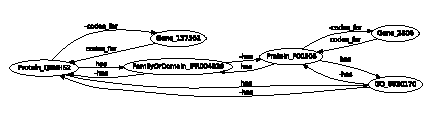
\includegraphics[width=16cm]{images/subgraph.pdf}
\caption{Подграф, состоящий из путей между похожими генами}
\label{subgraph}
\end{figure}

Существует большое количество биологических баз данных с открытым доступом, информация в которых может быть представлена как помеченный граф, в котором вершины соответствуют сущностям (протеины, гены, фенотипы), а рёбра отношениям между ними (взаимодействует, кодирует). Пути между вершинами позволяют найти новые связи в данных, либо показывают уже известные отношения. Подграф, построенный на всех найденных путях, более наглядно демонстрирует связи между вершинами.

Реальный набор биологических данных был собран из разных баз данных, находящихся в открытом доступе:  Entrez Gene (информация о генах) \cite{entrezgene}, UniProt (протеины) \cite{uniprot}, Gene Ontology (биологические процессы) \cite{geneontology}, STRING (связи между протеинами) \cite{string}, InterPro (семейства белков) \cite{interpro}, KEGG (связи между генами) \cite{kegg}, HomoloGene (группы гомологий генов) \cite{homologene}. Данные были ограничены набором из пяти организмов: Homo sapiens, Rattus norvegicus, Mus musculus, D. melanogaster и C. elegans. Объединенные в один файл данные состоят из троек: субъект, отношение, объект. Такие тройки образуют помеченный ориентированный граф.
\subsection{Запросы}

\begin{figure}
$$
\begin{array}{crcl}
&\mbox{\texttt{ [<Start>] }} \\
&\mbox{\texttt{s}} &:& \mbox{\texttt{gene }} \\
&\mbox{\texttt{v}} &:& \mbox{\texttt{protein | gene | GO | PATHWAY | FAMDOM}} \\
&&&\mbox{\texttt{| HOMOLOGENE}} \\
&\mbox{\texttt{similar}} &:& \mbox{\texttt{CODESFOR v RCODESFOR | BELONGS v RBELONGS}} \\
&&&\mbox{\texttt{| HAS v RHAS | HOMOLOGTO v RHOMOLOGTO}} \\
&\mbox{\texttt{protein}} & :& \mbox{\texttt{protein similar PROTEIN | PROTEIN}} \\
&\mbox{\texttt{gene}} & :& \mbox{\texttt{gene similar GENE | GENE}} \\
\end{array}
$$
\caption{Грамматика на языке YARD, задающая похожие гены}
\label{grammar}
\end{figure}

\begin{figure}
$$
\begin{array}{crcl}
&\mbox{\texttt{ [<Start>] }} \\
&\mbox{\texttt{s}} &:& \mbox{\texttt{gene }} \\
&\mbox{\texttt{v}} &:& \mbox{\texttt{protein | gene | GO | PATHWAY | FAMDOM}} \\
&&&\mbox{\texttt{| HOMOLOGENE}} \\
&\mbox{\texttt{similar}} &:& \mbox{\texttt{CODESFOR v RCODESFOR | BELONGS v RBELONGS}} \\
&&&\mbox{\texttt{| HAS v RHAS | HOMOLOGTO v RHOMOLOGTO}} \\
&\mbox{\texttt{ps}} & :& \mbox{\texttt{ (PROTEIN similar) *[1..2]}} \\
&\mbox{\texttt{protein}} & :& \mbox{\texttt{ps PROTEIN | PROTEIN}} \\
&\mbox{\texttt{gs}} & :& \mbox{\texttt{(GENE similar) *[1..2]}} \\
&\mbox{\texttt{gene}} & :& \mbox{\texttt{gs GENE | GENE}} \\
\end{array}
$$
\caption{Итоговая грамматика с ограничениями, задающая похожие гены}
\label{finalgrammar}
\end{figure}

Все вершины в полученном графе имеют уникальную метку. Но для удобства будем различать их по типу: гены, фенотипы и т.д. Назовём две вершины в графе похожими, если они одного типа и имеют рёбра одного типа к похожим вершинам. Это определение рекурсивно. Таким образом, путь между похожими вершинами представляет собой палиндром, который нельзя задать с помощью регулярной грамматики. 

На рисунке \ref{grammar} показана КС-грамматика на языке YARD, задающая класс путей, в которых начальный и конечный терминалы являются похожими генами. Для поиска похожих генов нетерминал gene, обозначающий последовательность похожих генов, указывается стартовым. Нетерминал similar задаёт отношение схожести генов и протеинов: существуют рёбра одного типа (например, BELONGS и RBELONGS) к похожим вершинам, которые обозначаются нетерминалом v.

В статье \cite{subgraph} при тестировании производительности длину путей ограничивали от 4 до 8. В алгоритме GLL в проекте YaccConstructor нет простого способа добавить такое ограничение. Поэтому, с целью уменьшения длины пути в грамматику были добавлены нетерминалы ps и gs, ограничивающие последовательность похожих протеинов и генов соответственно от одного до двух. На рисунке \ref{finalgrammar} показана итоговая грамматика с описанными выше ограничениями, задающая похожие гены.

На рисунке \ref{subgraph} показан подграф, который является результатом выполнения описанного выше запроса на небольших входных данных. Данный подграф содержит пути между похожими генами $Gene\_2806$ и $Gene\_137362$. Из рисунка видно, что эти гены кодируют похожие протеины, которые имеют рёбра одного типа $has$ и $-has$ к одним и тем же вершинам $FamilyOrDomain\_IPR004839$ и $GO\_0030170$. То есть гены удовлетворяют описанному определению похожих вершин.

\subsection{Производительность}

\begin{figure}
\begin{center}
\begin{tikzpicture}
\begin{axis}[
    xlabel = {Количество рёбер, тыс},
    ylabel = {Время, с},
    legend style={at={(0.5,-0.3)},anchor=north}
]
\addplot coordinates {
  (1.048,0.118) (2.334,0.57) (4.742,2.92) (7.046,7.72) (9.850,15.12) (12.398,27) (14.968,43) (17.432,69.7) (20.480,108.5)
};
\addplot coordinates {
  (1.048,0.134) (2.334,0.56) (4.742,2.97) (7.046,8.05) (9.850,17.45) (12.398,26.3) (14.968,42.5) (17.432,73) (20.480,107.5)
};
\legend{ 
  с метками на вершинах, 
  без меток на вершинах
};
\end{axis}
\end{tikzpicture}
\end{center}
\caption{Время работы алгоритма}
\label{time}
\end{figure}

Для оценки производительности была проведена серия экспериментов. Результаты приведены на графике, изображённом на рисунке \ref{time}. В статье \cite{subgraph} был проведён похожий эксперимент, но длины путей были ограничены от 4 до 8. В данной работе добиться такого ограничения не удалось, подграф строится по путям любой длины, поэтому нет возможности напрямую сравнить результаты.

Также была произведена серия экспериментов для сравнения производительности с алгоритмом GLL для графов без меток на вершинах. Замеры проведены на тех же данных, но с предварительным преобразованием графа в вершинно--рёберной граф (вершины с метками заменяются на рёбра). Результаты приведены на рисунке \ref{time}. Из графика видно, что выполнение запроса двумя способами занимает примерно одинаковое количество времени.

Таким образом, эксперименты показали, что реализованный алгоритм работает за приемлемое время на графах с числом рёбер до 20 тысяч. По сравнению с алгоритмом для графов с метками только на рёбрах выигрыша нет. Однако реализованный алгоритм избавляет от необходимости преобразовывать граф в вершинно--рёберный, что позволяет сэкономить ресурсы при больших входных данных.

\section{Заключение}
В ходе работы получены следующие результаты:
\begin{itemize}
    \item реализована возможность поиска путей в графе с помеченными вершинами и рёбрами по заданной КС-грамматике;
    \item написаны тесты;
    \item реализован интерфейс для получения и обработки результатов;
    \item проведены экспериментальные исследования.
\end{itemize}

\subsection{Дальнейшее направление работ}

Как показали результаты экспериментов, выполнение КС-запросов к графам уже с 20 тысячами рёбер занимает больше 100 секунд. Для уменьшения времени работы алгоритма и для выполнения запросов к графам большего размера исследовать возможность ограничения длины искомых путей в реализованном алгоритме GLL в YaccConstructor.

\setmonofont[Mapping=tex-text]{CMU Typewriter Text}
\bibliographystyle{ugost2008ls}
\bibliography{diploma.bib}
\end{document}
